% Editable reconstruction; interpretation recorded in root.json.
% Shared standalone design for the editable figure reconstructions.
\documentclass[tikz,border=5pt,10pt]{standalone}
\usepackage[T1]{fontenc}
\usepackage[utf8]{inputenc}
\usepackage{newpxtext,newpxmath}
\usepackage[scaled=.94]{sourcesanspro}
\usepackage{pgfplots}
\pgfplotsset{compat=1.18}
\usetikzlibrary{arrows.meta,calc,positioning,decorations.pathreplacing,
  decorations.markings,patterns,matrix,shapes.geometric,fit,backgrounds,
  intersections,angles,quotes}
\definecolor{ink}{HTML}{203746}
\definecolor{accent}{HTML}{146C78}
\definecolor{muted}{HTML}{667780}
\definecolor{signalred}{HTML}{B94B44}
\color{ink}
\tikzset{>=Latex,line width=.8pt,
  every node/.style={font=\small},
  axis/.style={->,draw=muted,line width=.5pt},
  guide/.style={draw=muted,dashed,line width=.45pt},
  curve/.style={draw=accent,line width=1pt},
  marker/.style={circle,fill=accent,inner sep=1.5pt},
  labelbox/.style={fill=white,inner sep=2pt}}

\begin{document}

\begin{tikzpicture}[x=1.35cm,y=1.05cm]
\draw[step=1,muted!15,very thin] (-3.5,-3.5) grid (3.5,3.5);
\draw[axis] (-3.75,0)--(3.85,0) node[right] {$u/T$};
\draw[axis] (0,-3.65)--(0,3.8) node[above] {$v=Q_T(u)$};
\draw[guide] (-3.5,-3.5)--(3.5,3.5);
\foreach \n in {-3,-2,-1,0,1,2,3}{
\draw[curve] ({\n-.5},\n)--({\n+.5},\n);
\fill[accent] ({\n-.5},\n) circle(2pt);
\draw[accent,fill=white] ({\n+.5},\n) circle(2pt);
\ifnum\n=0\else\node[below=3pt,fill=white,inner sep=1pt] at (\n,0) {$\n$};\node[left=3pt,fill=white,inner sep=1pt] at (0,\n) {$\n$};\fi}
\node[fill=white,align=center] at (-1.9,2.5) {$v-\tfrac12\leq u/T<v+\tfrac12$\\[3pt]$D_T(v)=Tv$};
\node[below=5pt] at (.5,0) {$\frac12$};
% A vertical error is measured at one fixed input, not along the diagonal.
\draw[signalred,<->,line width=1pt] (1.35,1)--(1.35,1.35);
\fill[signalred] (1.35,1) circle(1.5pt);
\fill[signalred] (1.35,1.35) circle(1.5pt);
\draw[signalred!70] (1.45,1.17)--(2.25,.55);
\node[font=\scriptsize,signalred,fill=white,inner sep=2pt] at (2.45,.43) {$|v-u/T|$};
\node at (0,-4.1) {$|D_T(Q_T(u))-u|\leq T/2$};
\end{tikzpicture}
\end{document}
